\documentclass[11pt]{article}
\usepackage[utf8]{inputenc} % Para caracteres en espa�ol
\usepackage{amsmath,amsthm,amsfonts,amssymb,amscd}
\usepackage{multirow,booktabs}
\usepackage[table]{xcolor}
\usepackage{fullpage}
\usepackage{lastpage}
\usepackage{enumitem}
\usepackage{multicol}
\usepackage{fancyhdr}
\usepackage{mathrsfs}
\usepackage{wrapfig}
\usepackage[final]{pdfpages}
\usepackage{setspace}
\usepackage{esvect}
\usepackage{calc}
\usepackage{multicol}
\usepackage{cancel}
\usepackage{graphicx}
\graphicspath{ {picturesC/} }
\usepackage[retainorgcmds]{IEEEtrantools}
\usepackage[margin=3cm]{geometry}
\usepackage{amsmath}
\newlength{\tabcont}
\setlength{\parindent}{0.0in}
\setlength{\parskip}{0.05in}
\usepackage{empheq}
\usepackage{framed}
%\usepackage{newtxmath}
\usepackage{euscript}
\DeclareMathAlphabet{\mathpzc}{T1}{pzc}{m}{it}
\usepackage[most]{tcolorbox}
\usepackage{xcolor}
\colorlet{shadecolor}{orange!15}
\parindent 0in
\parskip 12pt
\geometry{margin=1in, headsep=0.25in}
\theoremstyle{definition}
\newtheorem{defn}{Definition}
\newtheorem{reg}{Rule}
\newtheorem{exer}{Exercise}
\newtheorem{note}{Note}
\newcommand{\volume}{{\ooalign{\hfil$V$\hfil\cr\kern0.08em--\hfil\cr}}}
\newcommand{\parr}{\mathbin{\|}} % Parralel Symbol
\begin{document}
\setcounter{section}{1}
\setcounter{page}{33}
\setcounter{equation}{64}
\def\thepart{\arabic{part}}
\setcounter{part}{7}
\numberwithin{equation}{part}

 \pagestyle{fancy}
\fancyhf{}
\rhead{Section 7:  Electrothermal Propulsion}
\rfoot{Page \thepage}
\thispagestyle{empty}

\begin{center}
{\LARGE \bf Section 7:  Electrothermal Propulsion}\\
{\large AE435}\\
Spring 2018
\end{center}
\vspace{5mm}
\section{Resistojets}
\vspace{25mm}
\tableofcontents
\newpage
Consider a small tube of diameter, D,  and length, L. One end is connected to a propellant reservoir through a valve, and the other is attached to a nozzle. The tube is being heated by resistive Joule heating.  A current, I, is being driven through the tube by a voltage/potential, V. Propellant is entering the tube with a constant mass flow rate, $\dot{m}$.
  \begin{center}
 \vspace{80mm}
 \begin{equation*}
\begin{aligned}
R = \frac{V}{I} \sim 1 \Omega
\end{aligned}
\end{equation*}
  \textbf{Figure 9:}
 \end{center}
We seek a model to predict the temperature change of the liquid between the entrance of the tube and the exit.
  \begin{center}
 \vspace{70mm}
  \textbf{Figure 10:}
 \end{center}

Simple model,	$h = C_p \, T$
 
The Ohmic heating of the tube over a length $\mathrm{d}x$ is:

\begin{equation}
\begin{aligned}
I^2 \, R \, \frac{\mathrm{d}x}{L}
\end{aligned}
\end{equation}
 
The heating of the propellant over a length dx is:
 
 \begin{equation}
\begin{aligned}
\dot{m} \, C_p \, \mathrm{d}T
\end{aligned}
\end{equation}
Equating these yields:
 \begin{equation}
\begin{aligned}
\frac{\mathrm{d}T}{\mathrm{d}x} = \frac{I^2 \, R}{\dot{m} \, C_p \, L} = \text{ constant}
\end{aligned}
\end{equation}
 
Integrating (7.67) from $0 \rightarrow x$,
 \begin{equation}
\begin{aligned}
T_{out} - T_{in} = \frac{I^2 \, R}{\dot{m} \, C_p} \, \frac{x}{L} 
\end{aligned}
\end{equation}
 
Control the change in temperature with mass flow rate,      $\dot{m}$	, and power input, $P = I^2 \, R = I \, V$.
 
 \begin{equation*}
\begin{aligned}
\frac{P}{\dot{m}} \quad \text{or} \quad  \Bigg[\frac{W}{kg/s}\Bigg] \quad \text{or} \quad\Bigg[\frac{J}{kg}\Bigg]
\end{aligned}
\end{equation*}
 
We can also analyze the heat transfer between the wall and the fluid/propellant.
 
 \begin{equation}
\begin{aligned}
\mathrm{d}\dot{Q} = \mathfrak{H} \, A \, \Delta T = \mathfrak{H} \, (\pi D \mathrm{d}x)(T_{wall} - T)
\end{aligned}
\end{equation}

 Where $\mathfrak{H}$ is the heat transfer coefficient, $\Big[\frac{W}{m^2 \, K}\Big]$
 
The heat put into the system as a result of the joule heating on the tube we are applying is...
  \begin{equation*}
\begin{aligned}
\mathrm{d}\dot{Q} = \frac{I^2 \, R}{L} \, \mathrm{d}x \qquad \text{(Ohmic heating in dx, Equation 7.65)}
\end{aligned}
\end{equation*}
Such that
 \begin{equation}
\begin{aligned}
(T_{wall} - T) = \Delta T_w =  \frac{I^2 \, R}{(\pi D L) \, \mathfrak{H}} = \text{constant}
\end{aligned}
\end{equation}
 \newpage
 If we wanted to plot these we get...
  \begin{center}
 \vspace{80mm}
  \textbf{Figure 11:}
 \end{center}
 
The ratio of convective heat transfer to conductive heat transfer is given by the Nusselt number:
 
 \begin{shaded}
 \textbf{Nusselt Number}
 \begin{equation}
\begin{aligned}
N_{u_D} = \frac{\mathfrak{H} \, D}{k_f}
\end{aligned}
\end{equation}
Where
 \begin{equation*}
\begin{aligned}
 \mathfrak{H} &= \text{Convective Heat Transfer Coefficient} & \qquad & \Bigg[\frac{W}{m ^2\, K}\Bigg]\\ \\
 D &= \text{Diameter} \qquad [m] &&\\ \\
 k_f &= \text{Thermal Conductivity of the Fluid} & \qquad & \Bigg[\frac{W}{m \, K}\Bigg]\\
\end{aligned}
\end{equation*}
 \end{shaded}
 
For Laminar flow, convection with uniform surface heat flux for a circular tube yields:
 \begin{equation*}
\begin{aligned}
N_{u_D} \cong 4.36
\end{aligned}
\end{equation*}

   %\noindent\makebox[\textwidth]{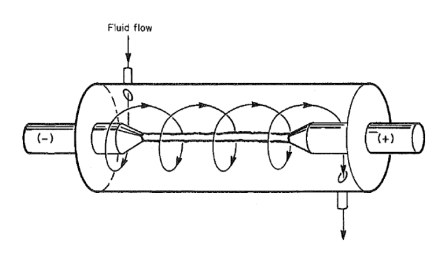
\includegraphics[scale=0.7]{11.png}}\\



\end{document}